% Outer measure on the line: two interval covers of the same set.
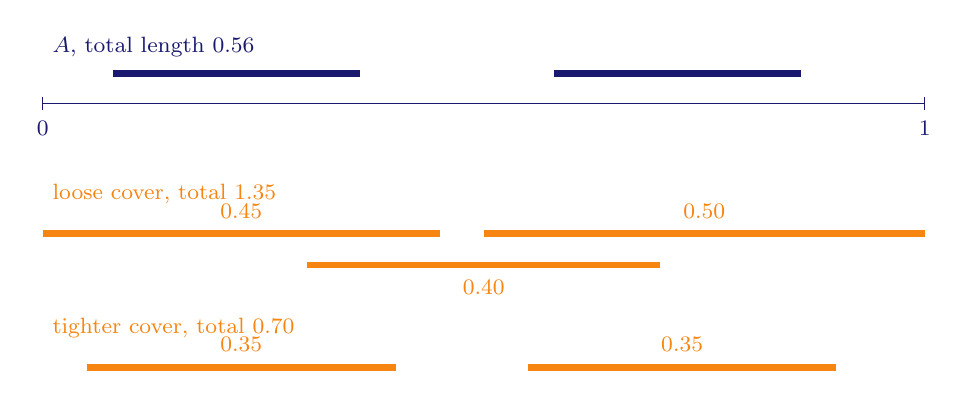
\begin{tikzpicture}[x=11.2cm,y=1.0cm,every node/.style={font=\footnotesize}]
  \draw[MidnightBlue] (0,0) -- (1,0);
  \draw[MidnightBlue] (0,-0.08) -- (0,0.08);
  \draw[MidnightBlue] (1,-0.08) -- (1,0.08);
  \node[MidnightBlue,below] at (0,-0.1) {$0$};
  \node[MidnightBlue,below] at (1,-0.1) {$1$};
  \draw[MidnightBlue,line width=2.8pt] (0.08,0.38) -- (0.36,0.38);
  \draw[MidnightBlue,line width=2.8pt] (0.58,0.38) -- (0.86,0.38);
  \node[MidnightBlue,anchor=west] at (0,0.72) {$A$, total length $0.56$};

  \node[BurntOrange,anchor=west] at (0,-1.15) {loose cover, total $1.35$};
  \draw[BurntOrange,line width=2.4pt] (0.00,-1.65) -- (0.45,-1.65);
  \draw[BurntOrange,line width=2.4pt] (0.30,-2.05) -- (0.70,-2.05);
  \draw[BurntOrange,line width=2.4pt] (0.50,-1.65) -- (1.00,-1.65);
  \node[BurntOrange,anchor=south] at (0.225,-1.58) {$0.45$};
  \node[BurntOrange,anchor=north] at (0.50,-2.12) {$0.40$};
  \node[BurntOrange,anchor=south] at (0.75,-1.58) {$0.50$};

  \node[BurntOrange,anchor=west] at (0,-2.85) {tighter cover, total $0.70$};
  \draw[BurntOrange,line width=2.4pt] (0.05,-3.35) -- (0.40,-3.35);
  \draw[BurntOrange,line width=2.4pt] (0.55,-3.35) -- (0.90,-3.35);
  \node[BurntOrange,anchor=south] at (0.225,-3.28) {$0.35$};
  \node[BurntOrange,anchor=south] at (0.725,-3.28) {$0.35$};
\end{tikzpicture}
